\input{doctools/latex/magazine_template.tex}   %Page setup
\input{doctools/latex/mycommands.tex}       %Some useful commands

% Figure search path
\graphicspath{
              {figs/} % Figures drawn with xfig
              {pngs/} % Other graphics files
}

% Use \draftnote to mark the filenames of figures
\newcommand{\isdraft}{1} %Choose 1 for draft, 0 for release

\begin{document}





%%%%%%%%%%%%%%%%%%%%%%%%%%%%%%%%%%%%%%%%%%%%%%%%%%%%%%%%%%%%%%%%%%%%
%Title
%%%%%%%%%%%%%%%%%%%%%%%%%%%%%%%%%%%%%%%%%%%%%%%%%%%%%%%%%%%%%%%%%%%%
\begin{center}
	{\huge ASCII command interface for the AVR Butterfly}\\
	\today
\end{center}

%%%%%%%%%%%%%%%%%%%%%%%%%%%%%%%%%%%%%%%%%%%%%%%%%%%%%%%%%%%%%%%%%%%%
%Table of contents
%%%%%%%%%%%%%%%%%%%%%%%%%%%%%%%%%%%%%%%%%%%%%%%%%%%%%%%%%%%%%%%%%%%%
\tableofcontents

\section{Introduction}
I love test equipment with open, well documented, ASCII command sets.  The plain text commands give a complicated-looking instrument a familiar interface, and beg you to use them in some clever measurement script.  Python's gnuplot and pySerial interfaces let you acquire and make pretty plots of your data -- all for free\cite{pyserial,gnuplot-py}. So when I need to automate hobby measurements at home, I immediately wish for an ASCII interface to whatever tool I'm measuring with.  This tool happens to be the AVR Butterfly board right now, simply because it's cheap and the LCD is handy.  

\clearpage
\section{Making connections to the Butterfly}
The AVR Butterfly board consists of an AVR ATmega169 microcontroller and some peripherals.  Figure \ref{fig:connections} shows the connections I make to it.  I only use 3 wires from the DB9 connector for serial communication with the PC -- there's no hardware handshaking.  And while I could also use this serial channel for programming, I find that using a dedicated programmer makes iterating my code much faster.  I thus solder a 6-pin header to the J403 position to use Atmel's AVRISP mkII programmer.  Finally, powering the board with an external supply at J401 means that I don't have to think about the Butterfly's button cell battery.  

\begin{figure}[ht]
    \begin{center}
        \includegraphics[clip,scale=1]{usart_pinout}
        \draftnote{usart\_pinout.fig}
        \caption{Connections needed for the AVR Butterfly.\label{fig:connections}}
    \end{center}
\end{figure}

\clearpage
\section{Handling incoming characters}
Characters are sent to the AVR via the USART connector shown in figure \ref{fig:connections}.  These characters trigger an interrupt service routine, which sorts them according to the flow shown in figure \ref{fig:recflow}.  Figure \ref{fig:recbuffer} illustrates the buffer characters are loaded into.  This inital step doesn't enforce any rules on command or argument sizes, provided that the total character count stays under the \texttt{RECEIVE\_BUFFER\_SIZE} limit.

When a combined string in the receive buffer is finished with a carriage return, the string is copied over to a second buffer.  I call this the parse buffer, since this is where the string will be searched for recognized commands and arguments.  Writing to this buffer must be prevented until its contents can be processed.  Sending commands faster than they can be processed will generate an error, and incoming commands will be dropped.  The maximum command processing frequency will depend on the system clock and other system tasks.  

\begin{figure}[ht]
    \begin{center}
        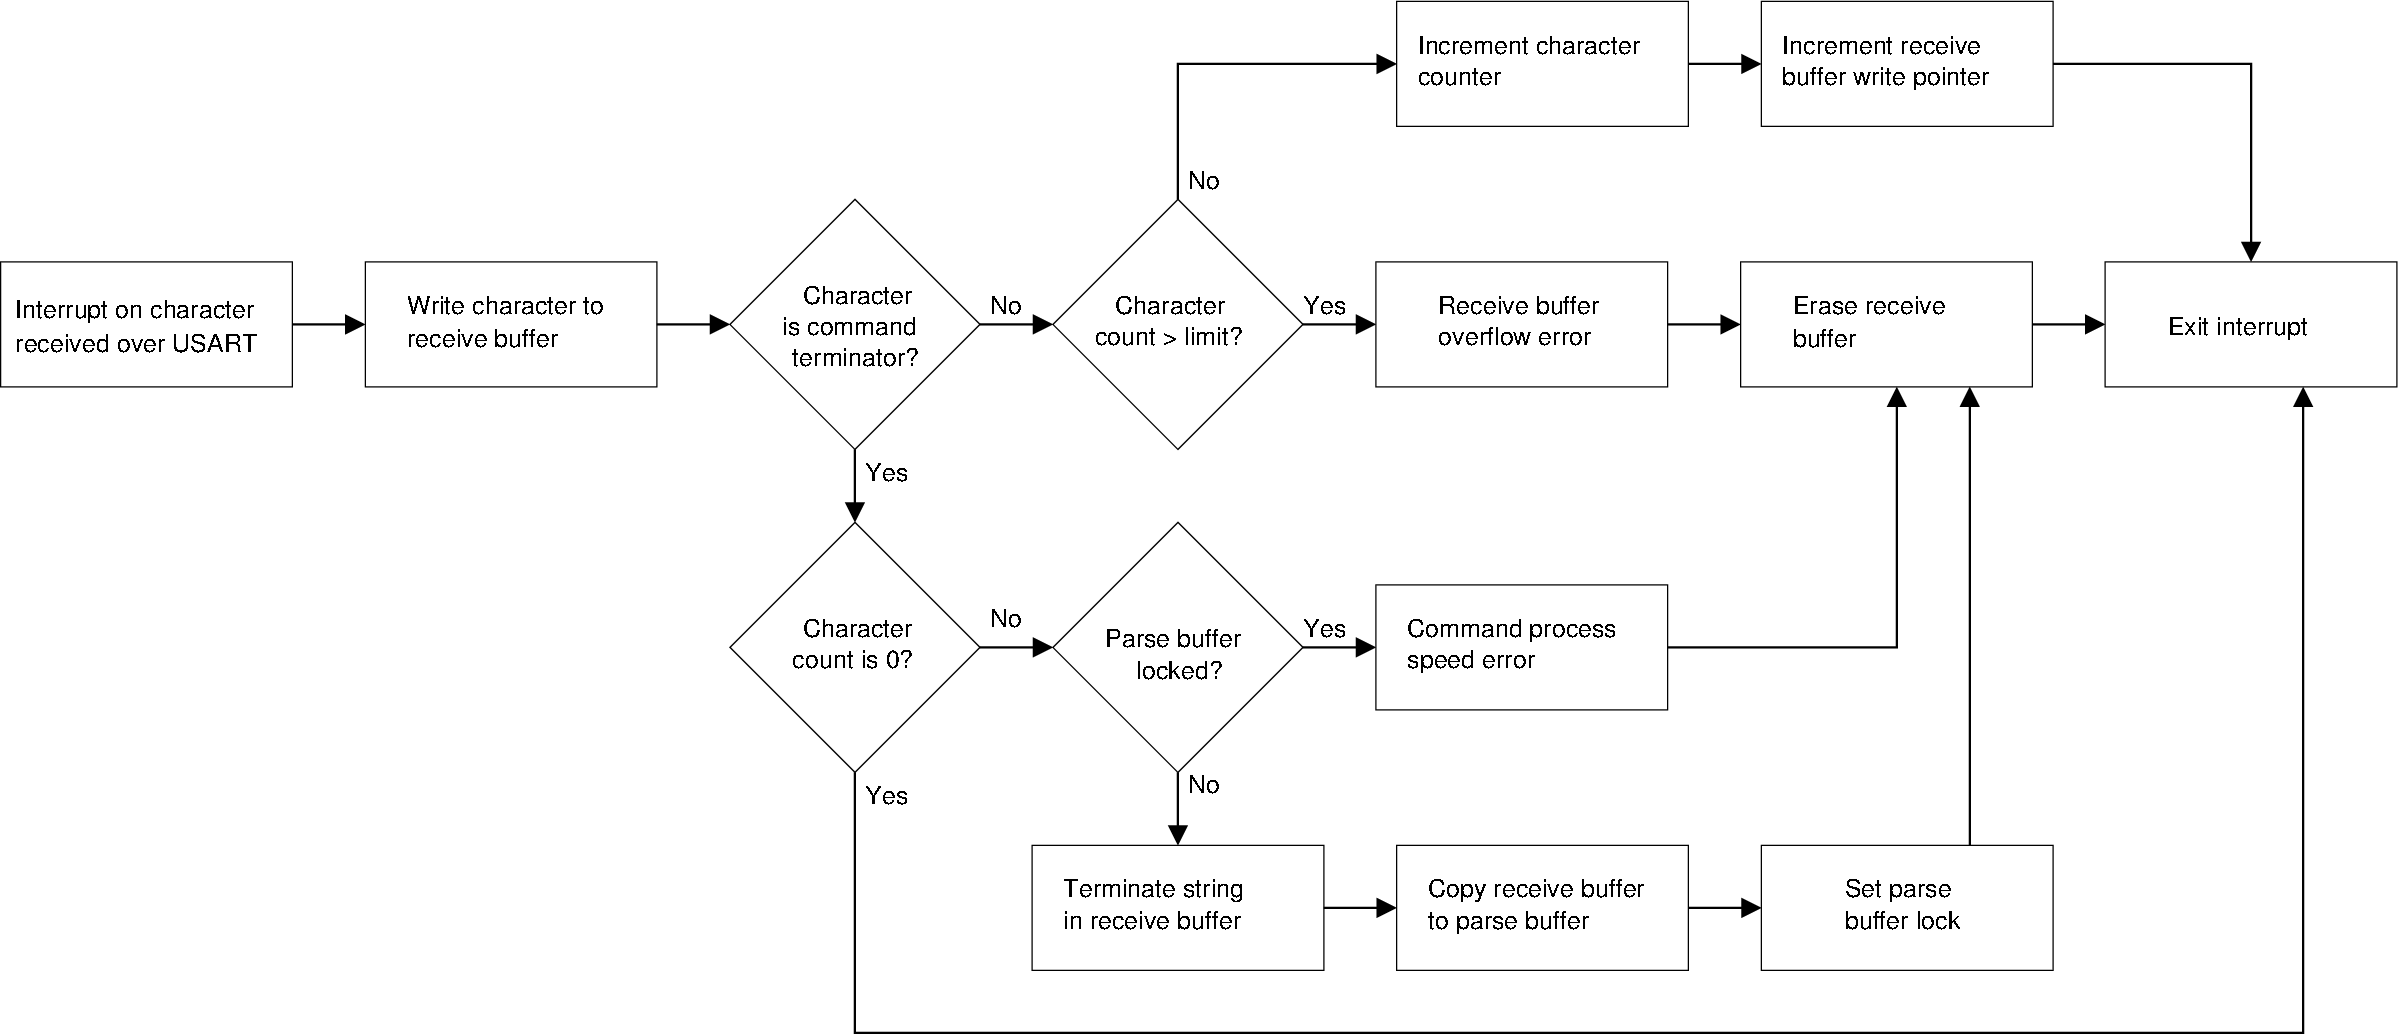
\includegraphics[clip,scale=0.45]{recv_cmd_flow}
        \draftnote{recv\_cmd\_flow.fig}
        \caption{Program flow for processing characters received over the Butterfly's USART.\label{fig:recflow}}
    \end{center}
\end{figure}

\begin{figure}[ht]
    \begin{center}
        \includegraphics[clip,scale=1]{recbuffer}
        \draftnote{recbuffer.fig}
        \caption{The received character buffer and pointers used to fill it.\label{fig:recbuffer}}
    \end{center}
\end{figure}

\clearpage{}
\section{Watching the progress}
I set up a logging system to help me understand how commands were being processed.  It's inconvienient to have the command and logging interfaces share the same communication channel, but the Butterfly only has one USART.  Reading command replies back without getting confused by general log messages will require some control over how the logging system works.  For now, figure \ref{fig:termgrab} shows the system processing the ``hello'' command with logging enabled at its most verbose level.  Each log message is tagged with a character representing the message severity (information, warning, error), followed by a string representing the subsystem responsible for the message.  These tags can be used to adjust what log messages should be suppressed, though I won't go into that here.  The ``Hello yourself!'' reply isn't a log message, and thus has no tags.

I should mention that these log message strings can easily overwhelm the Butterfly's RAM if they're not stored and referenced in flash memory.  Savannah\cite{url:savannah:pgmspace} and Dean Camera\cite{url:deancamera:pgmspace} have written great instructions for using the pgmspace module to handle this problem.

% See the termgrab.sh script for details about creating grab.eps
\begin{figure}[ht]
    \begin{center}
        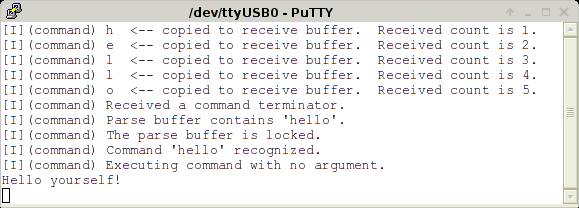
\includegraphics[clip,scale=0.5]{grab.eps}
        \draftnote{grab.eps}
        \caption{Terminal output showing the reception of and the reply to the ``hello'' command.\label{fig:termgrab}}
    \end{center}
\end{figure}




\clearpage{}
\section{Recognizing commands}
After finished combined strings are copied to the parse buffer, the system separates them into command and argument strings using the flow shown in figure \ref{fig:cmdflow}.


 searches through an array of understood commands for a match.  Listing \ref{lst:cmdarray} shows the array with definitions for the ``hello,'' ``logreg,'' and ``help'' commands.    The last element must be distinctive, so that routines scanning through the array will know when to stop.
 

% The command array figure is created with two text files (command_array.txt
% and command_type.txt) individually converted to fig format using code2fig.sh
% and then combined into one fig file.
\begin{listing}[ht]
    \begin{center}
        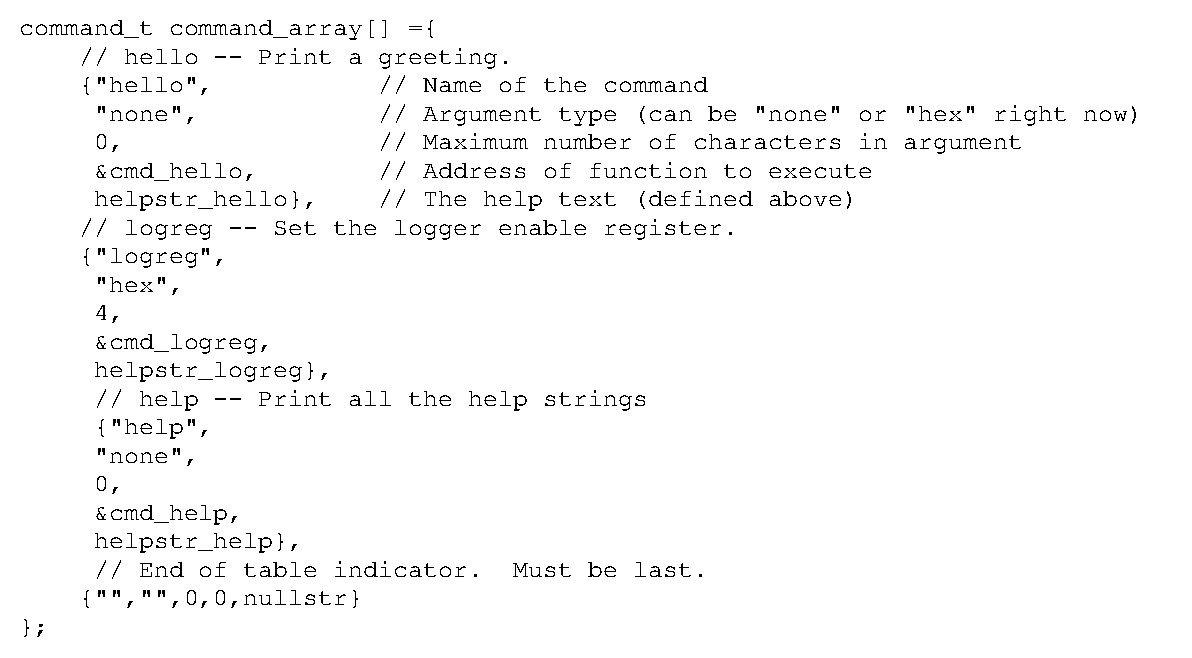
\includegraphics[clip,scale=0.75]{command_array}
        \draftnote{command\_array.fig}
        \caption{Commands are added to the system by adding to this array of command types.\label{lst:cmdarray}}
    \end{center}
\end{listing}

The command array structure is largely drawn from White\cite{bok:white2012}.



\clearpage{}
\section{The received character flow}








\clearpage{}
\section{The command processing flow}

\begin{figure}[ht]
    \begin{center}
        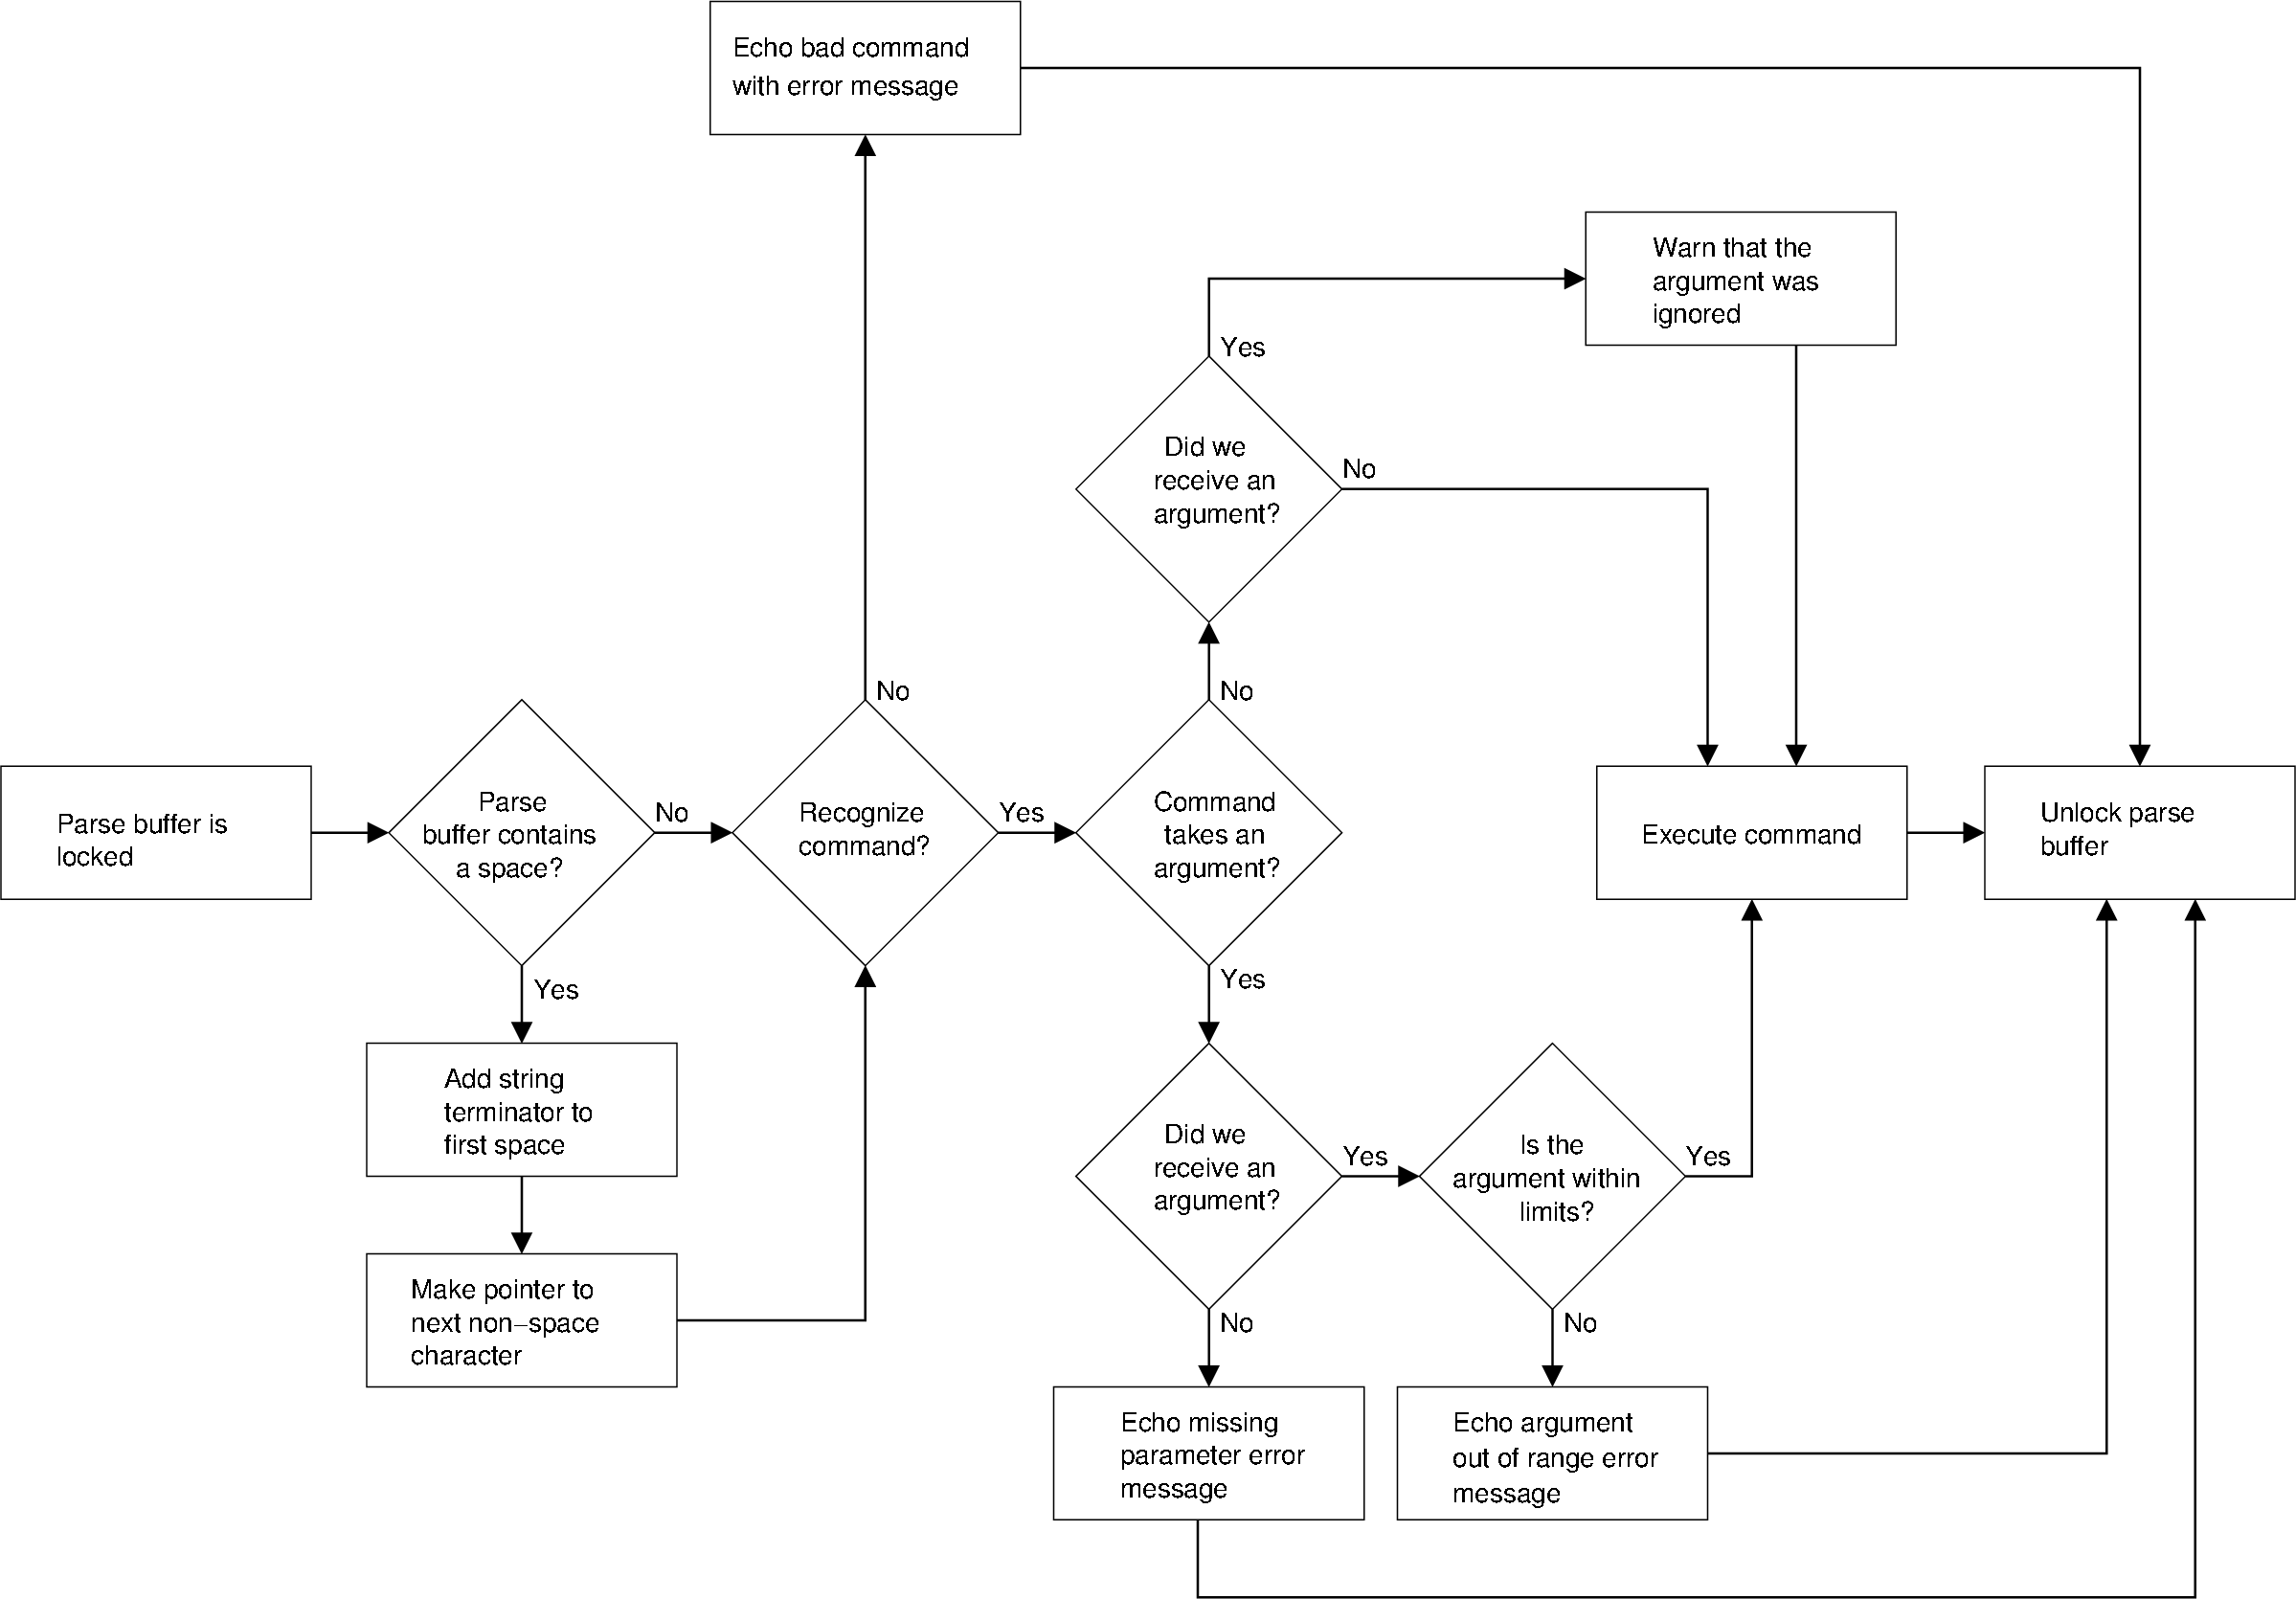
\includegraphics[clip,scale=0.5]{parse_cmd_flow}
        \caption{Program flow for processing fully-formed commands.\label{fig:cmdflow}}
    \end{center}
\end{figure}




\bibliography{doctools/latex/hydrorefs}
\end{document}
